% Copyright (C)  2020 Alain Matthes
% This work may be distributed and/or modified under the
% conditions of the LaTeX Project Public License, either version 1.3
% of this license or (at your option) any later version.
% The latest version of this license is in
%   http://www.latex-project.org/lppl.txt
% and version 1.3 or later is part of all distributions of LaTeX
% version 2005/12/01 or later.
% This work has the LPPL maintenance status `maintained'.
% The Current Maintainer of this work is Alain Matthes

% ``TKZdoc-fct-main '' is the french  documentation of tkz-fct.

\documentclass[DIV         = 14,
               fontsize    = 10,
               headinclude = false,
               index       = totoc,
               footinclude = false,
               twoside,
               headings    = small
               ]{tkz-doc-zh}
\usepackage{etoc}
\gdef\tkznameofpack{tkz-fct}
\gdef\tkzversionofpack{1.4c}
\gdef\tkzdateofpack{2020/05/05}
\gdef\tkznameofdoc{doc-tkz-fct}
\gdef\tkzdateofdoc{2020/05/05}
\gdef\tkzversionofdoc{1.4c}
\gdef\tkzauthorofpack{Alain Matthes}
\gdef\tkzauthoroftran{耿楠}
\gdef\tkzadressoftran{陕西$\cdot$杨凌}
\gdef\tkzadressofauthor{}
\gdef\tkznamecollection{AlterMundus}
\gdef\tkzurlauthor{http://altermundus.fr}
\gdef\tkzurlauthorcom{http://altermundus.fr}
\gdef\tkzengine{xelatex}
\def\nogreekalph{}
\usepackage{tkz-tab,tkz-fct}
\usepackage[english]{alterqcm}
\usepackage{tkz-euclide}
\usetikzlibrary{shapes.geometric}
\usepackage[colorlinks]{hyperref}
\hypersetup{
      linkcolor=Gray,
      citecolor=Green,
      filecolor=Mulberry,
      urlcolor=NavyBlue,
      menucolor=Gray,
      runcolor=Mulberry,
      linkbordercolor=Gray,
      citebordercolor=Green,
      filebordercolor=Mulberry,
      urlbordercolor=NavyBlue,
      menubordercolor=Gray,
      runbordercolor=Mulberry,
      pdfsubject={Graph function with gnuplot},
      pdfauthor={\tkzauthorofpack},
      pdftitle={\tkznameofpack},
      pdfkeywords={tikz, pgf, pdf, pdflatex, graphic, euclide,lualatex,
      points, maths, graph, gnuplot, angle ,function},
      pdfcreator={\tkzengine}
}
\usepackage{url}
\def\UrlFont{\small\ttfamily}
%
% \usepackage{fontspec}
% \setmainfont{texgyrepagella}[
%   Extension = .otf,
%   UprightFont = *-regular ,
%   ItalicFont  = *-italic  ,
%   BoldFont    = *-bold    ,
%   BoldItalicFont = *-bolditalic ,
% ]
% \setsansfont{texgyreheros}[
%   Extension = .otf,
%   UprightFont = *-regular ,
%   ItalicFont  = *-italic  ,
%   BoldFont    = *-bold    ,
%   BoldItalicFont = *-bolditalic ,
% ]
% \setmonofont{lmmono10-regular.otf}[
%   Numbers={Lining,SlashedZero},
%   ItalicFont=lmmonoslant10-regular.otf,
%   BoldFont=lmmonolt10-bold.otf,
%   BoldItalicFont=lmmonolt10-boldoblique.otf,
% ]
% \newfontfamily\ttcondensed{lmmonoltcond10-regular.otf}
%% (La)TeX font-related declarations:
\linespread{1.05}      % Pagella needs more space between lines
\usepackage{unicode-math}
\usepackage{fourier-otf}
\usepackage{tkzexample}
\usepackage{rotating,fancyvrb}
% \usepackage[english]{babel}
% \usepackage[autolanguage]{numprint}

\usepackage{microtype}
% \DisableLigatures{encoding = T1,
                  % family   = tt*}
\usepackage[parfill]{parskip}
\usepackage{array,multirow,multido,booktabs}
\usepackage{shortvrb,fancyvrb}
\usepackage{ipa}
\usepackage{csquotes}
\usepackage{pgfornament}
\makeatletter
\renewcommand*\l@subsubsection{\bprot@dottedtocline{3}{3.8em}{4em}}
\makeatother
\AtBeginDocument{\MakeShortVerb{\|}}

\RequirePackage{makeidx}
%\@twocolumnfalse
\makeindex
\newcommand*{\E}{\ensuremath{\mathrm{e}}}
\colorlet{graphicbackground}{white}
\colorlet{codebackground}{Gray!10}
% \usepackage[saved]{tkzexample}
% \def\tkzFileSavedPrefix{tkzFct}
\def\blue{\color{blue}}
\def\red{\color{red}}

% 分文档翻译,方便定位错误,加快编译速度
%必须是document环境的前最后一行代码
\usepackage{subfiles}

\begin{document}

%<--------------------- Première page présentation  ------------------------–>
\title{\tkznameofpack}
\date{\today}
\clearpage
\thispagestyle{empty}
\maketitle
\null
\makeatletter
\typeout{Load pgfornament font}
\AddToShipoutPicture*{%
\setlength\unitlength{1mm}
\put(70,120){%
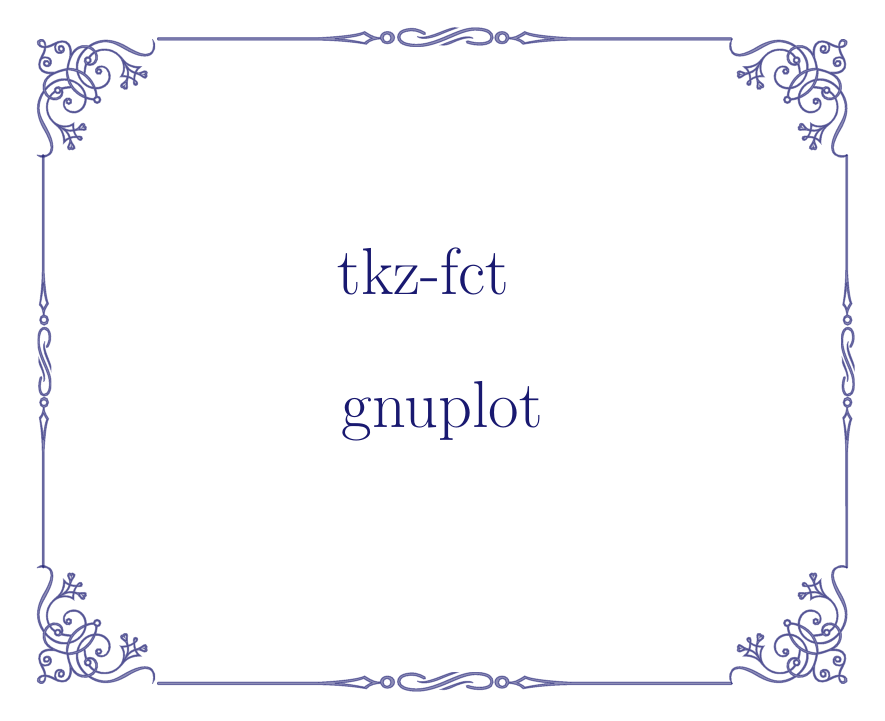
\begin{tikzpicture}
  \coordinate (A) at (0pt,240pt);
  \coordinate (B) at (300pt,240pt);
  \coordinate (C) at (300pt,0pt);
  \coordinate (D) at (0pt,0pt);
  \begin{scope}[opacity=0.5] % for opacity
    \pgfornamentline[color=MidnightBlue]{[xshift=1.65cm,yshift=-1mm]A}{[xshift=-1.58cm,,yshift=-1mm]B}{1}{88}; % AB
    \pgfornamentline[color=MidnightBlue]{[xshift=1.65cm,yshift=1.5mm]D}{[xshift=-1.58cm,yshift=1.5mm]C}{1}{88};
    \pgfornamentline[color=MidnightBlue]{[xshift=2.2mm,yshift=-1.59cm]A}{[xshift=2.2mm,yshift=1.59cm]D}{1}{88};
    \pgfornamentline[color=MidnightBlue]{[xshift=-1.2mm,yshift=-1.59cm]B}{[xshift=-1.2mm,yshift=1.59cm]C}{1}{88};
  \end{scope}
  \node[anchor=north west] at (A) {\pgfornament[color=MidnightBlue,opacity=0.5,width=1.5cm]{61}}; % A
  \node[anchor=north east] at (B) {\pgfornament[color=MidnightBlue,opacity=0.5,width=1.5cm,symmetry=v]{61}};% B
  \node[anchor=south east] at (C) {\pgfornament[color=MidnightBlue,opacity=0.5,width=1.5cm,symmetry=c]{61}}; % C
  \node[anchor=south west] at (D) {\pgfornament[color=MidnightBlue,opacity=0.5,width=1.5cm,symmetry=h]{61}}; % D
  \node[text width=280pt] at (150 pt,120 pt){%
  \begin{center}
    \color{MidnightBlue}
    \fontsize{24}{48}
    \selectfont tkz-fct宏包\par
                基于\tkzname{gnuplot}和\TIKZ{}的\par
                二维函数曲线绘图宏包
  \end{center}};
\end{tikzpicture}}}
\makeatother
\clearpage
\tkzSetUpColors[background=white,text=darkgray]

\nameoffile{\tkznameofpack}

\defoffile{
% \textbf{tkz-fct.sty  (v1.4c)} est un package pour créer à l'aide de \TIKZ,  des représentations graphiques de fonctions en 2D le plus simplement possible. Il est dépendant de \TIKZ\ et fera partie d'une série de modules ayant comme point commun, La création de dessins utiles dans l’enseignement des mathématiques. Ce sont des représentations du type scolaire qui correspondent à l’enseignement proposé dans les lycées français.
\textbf{tkz-fct.sty(v1.4c)}是一个基于\tkzname{gnuplot}和\TIKZ{}设计的用于绘制二维函数曲线的宏包,
它语法简单、使用方便,是\textbf{tkz-}系列宏包的一个模块,主要用于绘制数学教学中的各类函数曲线,
这些函数曲线符合法国高中教学的需求。
}

\presentation

\vspace*{24pt}
% \noindent\lefthand\ Je souhaite remercier \tkzimp{Till Tantau} pour avoir créé le merveilleux outil \tkzname{\TIKZ}, ainsi que \tkzimp{Michel Bovani} pour \tkzname{fourier}, dont l'association avec \tkzname{utopia} est excellente.

\noindent\lefthand\ 在此,要感谢\tkzimp{Till Tantau}开发了精彩的\tkzname{\TIKZ}宏包,
也要感谢\tkzimp{Michel Bovani}开发的\tkzname{fourier}宏包, 
这些宏包都能与\tkzname{utopia}宏包很好的协同工作。


\vspace*{12pt}
% \noindent\lefthand\ Je souhaite remercier aussi  \tkzimp{David Arnold} qui a corrigé un grand nombre d'erreurs et qui a testé de nombreux exemples, \tkzimp{Pablo González Luengo } pour son aide sur la documentation et la gestion du dépôt "GitHub", \tkzimp{Wolfgang Büchel} qui a corrigé également des erreurs et a construit de superbes scripts pour obtenir les fichiers d'exemples,  \tkzimp{John Kitzmiller}  et ses exemples, et enfin  \tkzimp{Gaétan Marris} pour ses remarques.

\noindent\lefthand\ 感谢\tkzimp{David Arnold},他纠正了宏包中许多错误,并对多数示例进行了测试;
感谢\tkzimp{Pablo González Luengo},他在Github仓库的文档管理方面提供全力的帮助;
感谢\tkzimp{Wolfgang Büchel},他也纠正了许多错误,并编写优秀的脚本管理示例文件;
感谢\tkzimp{John Kitzmiller},他设计并测试了更多的示例;
最后要感谢\tkzimp{Gaetan Marris},他的评论为宏包的改进提供了很好的思路。

% \vspace*{12pt}
% \noindent\lefthand\ Vous trouverez bientôt de nombreux exemples sur mon site~:
% \href{http://altermundus.fr}{altermundus.fr}

\vfill
% Vous pouvez envoyer vos remarques, et les rapports sur des erreurs que vous aurez constatées à l'adresse suivante~: \href{mailto:al.ma@mac.com}{\textcolor{blue}{Alain Matthes}}.
\noindent\lefthand\ 如果发现该文档的错误或有其他任何意见和建议,请发信至:\href{mailto:al.ma@mac.com}{\textcolor{blue}{Alain Matthes}}.

\noindent\lefthand\ 如果发现译文的错误或其有他任何意见和建议,请发信至:\href{mailto:nangeng@nwafu.edu.cn}{\textcolor{blue}{耿楠}}.

% This work may be distributed and/or modified under the
% conditions of the LaTeX Project Public License, either version 1.3
% of this license or (at your option) any later version.
可以在\href{http://www.ctan.org/}{CTAN}发布的``LATEX Project Public
License''协议下发布和修改该文档。
% <--------------------------------------------------------------------------->

\clearpage
\tableofcontents

\clearpage
\newpage

\setlength{\parskip}{1ex plus 0.5ex minus 0.2ex}
%<---------------------------- the files ------------------------------------>
\subfileinclude{chap00/TKZdoc-fct-why}
\subfileinclude{chap01/TKZdoc-fct-compilation}
\subfileinclude{chap02/TKZdoc-fct-installation}
\subfileinclude{chap03/TKZdoc-fct-fonctions}
\subfileinclude{chap04/TKZdoc-fct-point}
\subfileinclude{chap05/TKZdoc-fct-label}
\subfileinclude{chap06/TKZdoc-fct-tangent}
\subfileinclude{chap07/TKZdoc-fct-area}
\subfileinclude{chap08/TKZdoc-fct-riemann}
\subfileinclude{chap09/TKZdoc-fct-asymptote}
\subfileinclude{chap10/TKZdoc-fct-param}
\subfileinclude{chap11/TKZdoc-fct-polar}
\subfileinclude{chap12/TKZdoc-fct-symbol}
\subfileinclude{chap13/TKZdoc-fct-example}
\subfileinclude{chap14/TKZdoc-fct-interpolation}
\subfileinclude{chap15/TKZdoc-fct-VDW}
\subfileinclude{chap16/TKZdoc-fct-bac}
\subfileinclude{chap17/TKZdoc-fct-fppgf}
\subfileinclude{chap18/TKZdoc-fct-faq}
\subfileinclude{chap19/TKZdoc-fct-liste}
%<--------------------------------------------------------------------------->
\clearpage\newpage
\printindex
\end{document}
